\documentclass{article}
\usepackage{amsmath}
\usepackage{mathtools}
\usepackage{gensymb}
\usepackage[a4paper,inner=1.5cm,outer=1.5cm,top=2cm,bottom=0.5cm]{geometry} 
\usepackage{xcolor}                    
\usepackage{tikz}                           
\usepackage{multicol}
\usepackage{hyperref}
\usepackage{pgfplots}
\usetikzlibrary{calc}
\usetikzlibrary{intersections}
\usetikzlibrary{intersections,calc,angles,quotes}
\usetikzlibrary{shapes,arrows,positioning,decorations.pathreplacing,calc}
\usetikzlibrary{calc,angles,positioning,intersections,quotes,decorations.markings}
\usepackage{tkz-euclide}
\usetikzlibrary{backgrounds}
\usetikzlibrary{calc,through}
\usetikzlibrary{angles}
\usetikzlibrary{fadings}
\usetikzlibrary{shapes.geometric}
\usetikzlibrary{shapes.symbols}
\usepackage{draftwatermark}
\usepackage{mathptmx}

\SetWatermarkText{\textcolor{black!20}{Mathema Shukur}}
\SetWatermarkFontSize{2 cm}
\usepackage[utf8]{inputenc}
\usepackage{fontspec}

\setmainfont{[Kalpurush.ttf]}
\newfontface{\en}{[Arial.ttf]} %%this is optional, if you want to use a secondary font. Any english font is supported
\newlength\Radius
\setlength\Radius{4cm}
\begin{document} 
	\Large
	\textcolor{red}{Welcome To} 
	\\
	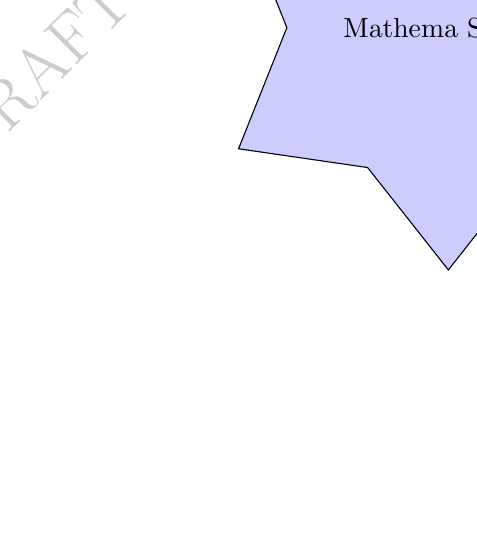
\begin{tikzpicture}
		\tikz \node [fill=blue!20,star,star points=6,draw] {Mathema Shukur };
	\end{tikzpicture}
	\\
	যাদের জন্যে প্রযোজ্যঃ  	\textcolor{magenta}{একাদশ ও দ্বাদশ শ্রেণীর শিক্ষার্থী} \\
	বিষয়ঃ \textcolor{magenta}{উচ্চতর গণিত ১ম পত্র} \\
	অধ্যায়ঃ \textcolor{magenta}{৪-বৃত্ত}\\ 
	\\
	\\
	(১)  মূল বিন্দুতে কেন্দ্র বিশিষ্ট বৃত্তের সমীকরণ  \\
	\\
	\textcolor{blue}{$x^2+y^2=r^2$}\\
	\\
	(২) নির্দিষ্ট কেন্দ্র ও ব্যাসার্ধ বিশিষ্ট বৃত্তের  সমীকরণ \\
	\\
	\textcolor{blue}{$(x-h)^2+(y-k)^2=r^2$}\\
	\\
	(৩) বৃত্তের সাধারণ সমীকরণ\\
	\\  
	\textcolor{blue}{$x^2+y^2+2gx+2fy+c=0$}\\
	\\
	(৪) ব্যাসের প্রান্ত বিন্দুদ্বয় $(x_1,y_1)$ এবং $(x_2,y_2)$ হলে বৃত্তের সমীকরণ\\
	\\ 
	\textcolor{blue}{$(x-x_1)(x-x_2)+(y-y_1)(y-y_2)=0$}\\
	\\
	(৫) একটি বৃত্ত \textcolor{blue}{$S=0$ }এবং একটি সরলরেখা \textcolor{blue}{$L=0$}  এর ছেদবিন্দুগামী বৃত্তের সমীকরণ  \textcolor{blue}{$S+kL=0$} \\
	\\
	(৬) দুইটি বৃত্ত \textcolor{blue}{$S_1=0$} ও \textcolor{blue}{$S_2=0$} এর ছেদবিন্দুগামী বৃত্তের সমীকরণ \textcolor{blue}{$S_1+kS_2=0$}\,\,[\textcolor{red}{$k\ne -1$}]\\  \\
	(৭) পোলার স্থানাঙ্কে বৃত্তের  সমীকরণ \\
	\textcolor{blue}{$r^2+2r(g\cos \theta+f\sin \theta )+c=0$}\\
	যেখানে 	$g=-\rho \cos \alpha,\,\,\,f=-\rho \sin \alpha,\,\,\,c=\rho^2-a^2 $\\
	\\ 
	একটি বৃত্তের সমীকরণ নির্ণয় কর যা $(-1,-2)$ বিন্দু এবং যা $\textcolor{blue}{x^2+y^2-8x-2y+7=0}$ বৃত্ত  ও  $\textcolor{blue}{x^2+y^2-4x+10y+8=0}$ বৃত্তের ছেদ বিন্দু দিয়ে যায়। \\ 
	\\
	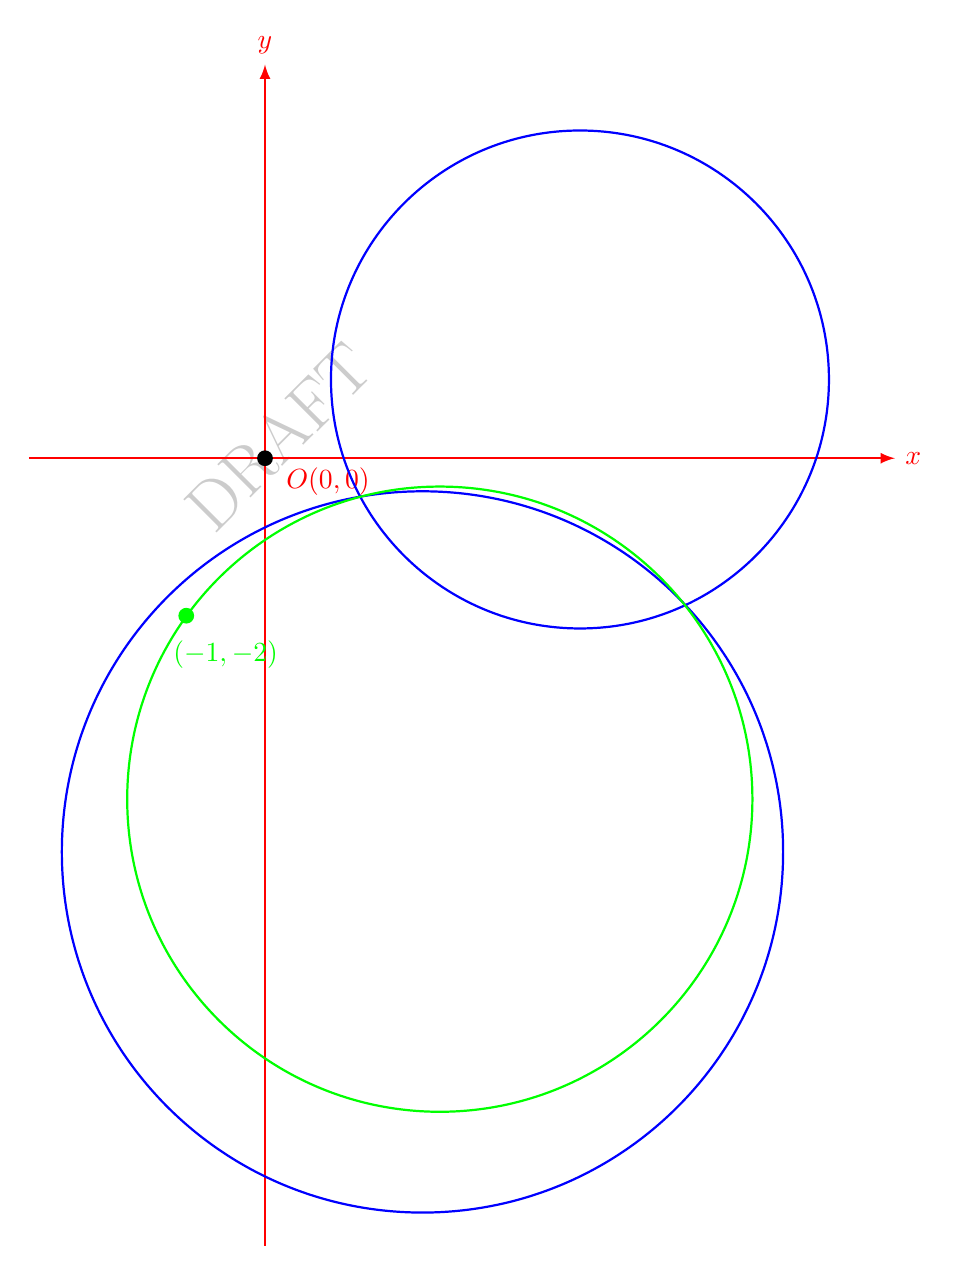
\begin{tikzpicture}[transform shape,scale=1]
		\draw [-latex,thick,red](-3,0) -- (8,0) node[right] {$x$} coordinate(x axis);
		\draw [-latex,thick,red](0,-10) -- (0,5) node[above] {$y$} coordinate(y axis);
		\fill[black] (0,0) circle (1 mm);
		\node at (0.8,-0.3) {$\textcolor{red}{O(0,0)}$};	
		\draw[thick,blue] (4,1) circle (3.162);
			\draw[thick,blue] (2,-5) circle (4.58);
				\draw[thick,green] (2.22,-4.33) circle (3.97);
					\fill[green] (-1,-2) circle (1 mm);
						\node at (-0.5,-2.5) {$\textcolor{green}{(-1,-2)}$};
	\end{tikzpicture}\\
	\\
	\begin{align*}
		S_1+kS_2&=0\,\,[\textcolor{red}{k\ne -1}]\\
		(x^2+y^2-8x-2y+7)+k(x^2+y^2-4x+10y+8)&=0\,\,[EQ01]\\
		\boxed{\textcolor{blue}{x=-1,\,\,y=-2}}&\\
	((-1)^2+(-2)^2-8(-1)-2(-2)+7)+k((-1)^2+(-2)^2-4(-1)+10(-2)+8)&=0\\
	1+4+8+4+7+k(1+4+4-20+8)&=0\\
		\\
	24+k(-3)&=0\\
	\\
	k&=8
	\end{align*}
	\\
	\begin{align*}
		(x^2+y^2-8x-2y+7)+k(x^2+y^2-4x+10y+8)&=0\,\,[EQ01]\\
		\boxed{\textcolor{blue}{k=8}}&\\
		(x^2+y^2-8x-2y+7)+8(x^2+y^2-4x+10y+8)&=0\\
		\\
	x^2+y^2-8x-2y+7+8x^2+8y^2-32x+80y+64&=0\\
	\\
	\textcolor{green}{9x^2+9y^2-40x+78y+71=0}&
	\end{align*}
\\
	একটি বৃত্তের সমীকরণ নির্ণয় কর যা  $\textcolor{blue}{x^2+y^2-x+7y-3=0}$ বৃত্ত  ও  $\textcolor{blue}{x^2+y^2-5x-y+1=0}$ বৃত্তের ছেদ বিন্দু দিয়ে যায় এবং যার কেন্দ্র $\textcolor{blue}{x+y=0}$ রেখার উপর অবস্থিত।\\  
	\\
	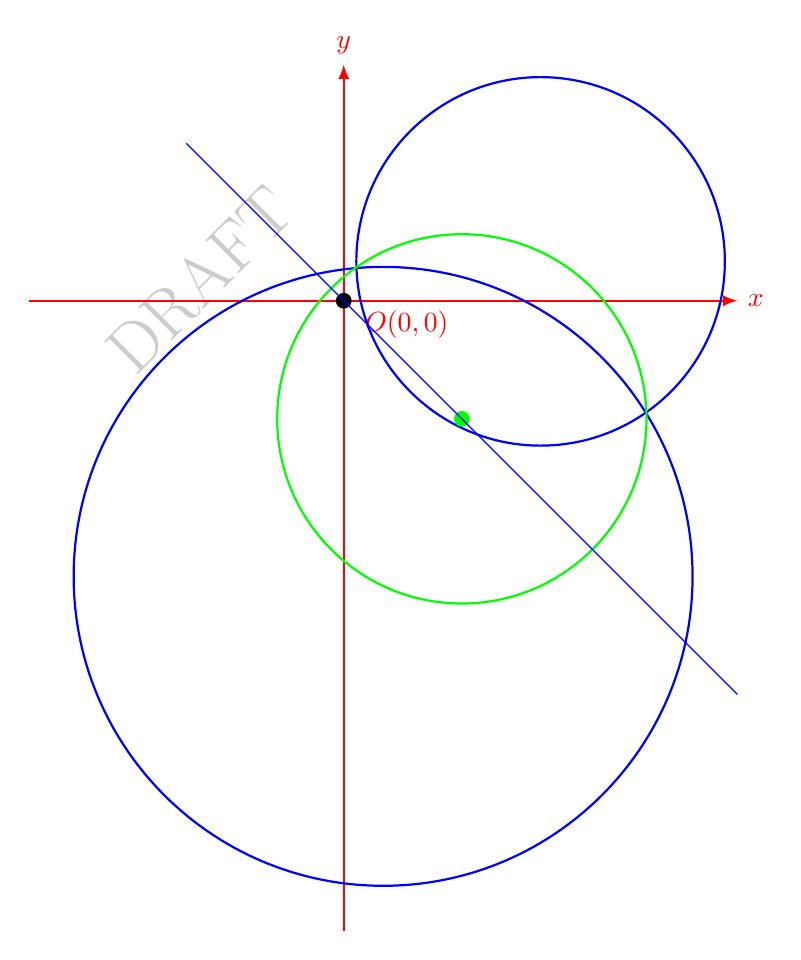
\begin{tikzpicture}[transform shape,scale=1]
	\draw [-latex,thick,red](-4,0) -- (5,0) node[right] {$x$} coordinate(x axis);
	\draw [-latex,thick,red](0,-8) -- (0,3) node[above] {$y$} coordinate(y axis);
	\fill[black] (0,0) circle (1 mm);
	\node at (0.8,-0.3) {$\textcolor{red}{O(0,0)}$};	
	\draw[thick,blue] (0.5,-3.5) circle (3.93);
	\draw[thick,blue] (2.5,0.5) circle (2.34);
	\draw[thick,green] (1.5,-1.5) circle (2.345);
	\fill[green] (1.5,-1.5) circle (1 mm);
	\draw[blue](-2,2)--(5,-5);
\end{tikzpicture}\\
	\\
	\begin{align*}
			S_1+kS_2&=0\,\,[\textcolor{red}{k\ne -1}]\\
			\\ 
		(x^2+y^2-x+7y-3)+k(x^2+y^2-5x-y+1)&=0\,\,[EQ01]\\
		\\
	x^2+y^2-x+7y-3+kx^2+ky^2-5kx-ky+k&=0\\
		\\
			(k+1)x^2+(k+1)y^2+(-5k-1)x+(7-k)y+(k-3)&=0\\
		\\
		x^2+y^2+\left(\frac{-5k-1}{k+1}\right)x+\left(\frac{7-k}{k+1}\right)y+\frac{k-3}{k+1}&=0\\
		\\
		x^2+y^2+2\left(-\frac{5k+1}{2(k+1)}\right)x+2\left(\frac{7-k}{2(k+1)}\right)y+\frac{k-3}{k+1}&=0\\
	\end{align*}
	কেন্দ্র $(-g,-f)=\left(-\left(-\frac{5k+1}{2(k+1)}\right),-\left(\frac{7-k}{2(k+1)}\right)\right)$; যা $x+y=0$ রেখার উপর অবস্থিত  \\
	\\
	\begin{align*}
		x+y&=0\\
		\\
		\frac{5k+1}{2(k+1)}+\frac{k-7}{2(k+1)}&=0\\
		\\
		5k+1+k-7&=0\\
		\\
	6k-6&=0\\
	\\
	k&=1
	\end{align*}
\begin{align*}
		(x^2+y^2-x+7y-3)+k(x^2+y^2-5x-y+1)&=0\,\,[EQ01]\\
		\\
		(x^2+y^2-x+7y-3)+1(x^2+y^2-5x-y+1)&=0\\
		\\
		x^2+y^2-x+7y-3+x^2+y^2-5x-y+1&=0\\
		\\
		2x^2+2y^2-6x+6y-2&=0\\
		\\
	\textcolor{green}{	x^2+y^2-3x+3y-1=0}&\\
\end{align*}
\\
\href{https://www.youtube.com/watch?v=afVjGQrIpDs}{\textcolor{blue}{বৃত্ত ও সরলরেখার ছেদবিন্দুগামী বৃত্তের সমীকরণ}}
\end{document}